\chapter{Methodology and Design \label{sec:methodology}}
\todo[inline]{Implementation: how was your experiment/project accomplished? 
Include enough details of your method and tooling that someone can easily replicate your results.
}

% PRELUDE
This chapter contains the design decision and steps taken to complete the testbed creation and testing. The project can broken into the three main areas of hardware, software and digital signal processing. 

\section{Hardware \label{sec:hardware}}

\subsection{Software Defined Radio \label{sec: SDRdongle}}
The fundamental hardware aspect for this project is the Software Defined Radio (SDR), specifically, the SDR receiver module. \todo{ADD SECTION LABELS} As mentioned in section 2,4, software defined radio technology has been recently experienced decreasing costs and proliferation (CITE!!!). Broadly, the testbed was designed to accomodate a potential range of USB-A capable SDR modules, with the capability initially tested on a low cost RTL-SDR, before progressing to later prototyping on higher end MODEL X.

\vspace{0.5cm} \noindent 
\textbf{1. RTL-SDR Prototyping}
The low cost RTL-SDR was chosen as the initial SDR module for testbed prototyping  due to its low cost and wide availability. The specifics of the RTL-SDR are stated in section 2.4 \todo{REF}, it was connected to the RPi5 and higher level M1 Mac along with a simple SMI antenna as seen in the figure below \ref*{fig:rtlSDR}. 

\begin{figure}[htbp]
    \centering
    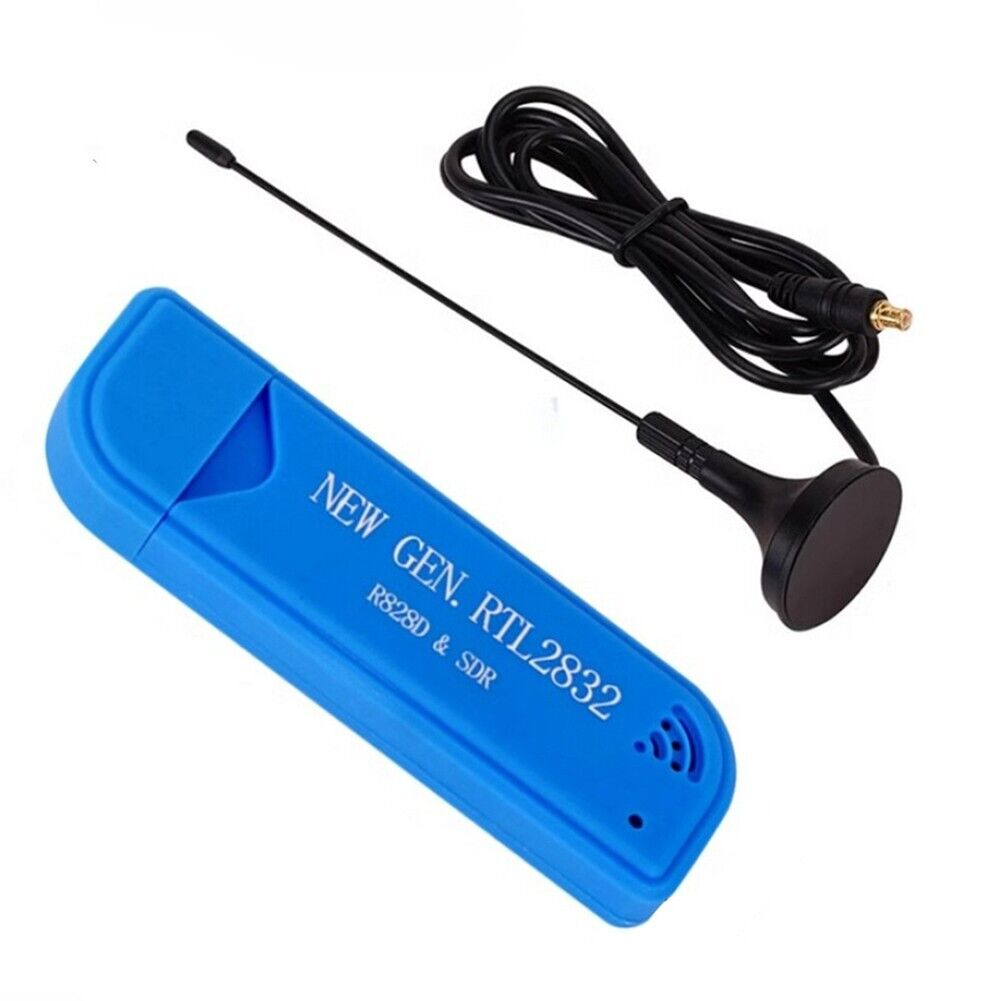
\includegraphics[width=0.3\textwidth]{rtlSdr.jpg}
    \caption{RTL-SDR with Simple SMA Antenna}
    \label{fig:rtlSDR}
\end{figure}

The RTL-SDR was tested with a range of software as mentioned in \ref*{label:SDRsoftware} to ensure hardware was correctly functioning and to gain familiarity with the process. 

\vspace{0.5cm} \noindent 
\textbf{2. MODEL X Implementation}

\todo[inline]{WHAT ARE THE SPECS OF SDR X}


\subsection{Embedded Computing Platform \label{sec:embedded computing}}
\subsection{NVME Based Storage \label{sec:storage}}
\subsection{Antenna Configuration \label{sec:antenna}}
\subsection{Testbed Design \label{sec:testbed}}


\section{Software}
\subsection{SDR Software \label{sec:SDRsoftware}}
\subsection{Networking Requirements \label{sec:networking}}


% METHOD FOR TESTING NOT THE ACTUAL RESULTS
\section{Digital Signal Processing Testing \& Simulation}



